\section{Příklad 4}
% Jako parametr zadejte skupinu (A-H)
\ctvrtyZadani{H}

Nejdříve si označíme směr smyčkových proudů v obvodu:
\begin{figure}[htb]
  \centering
  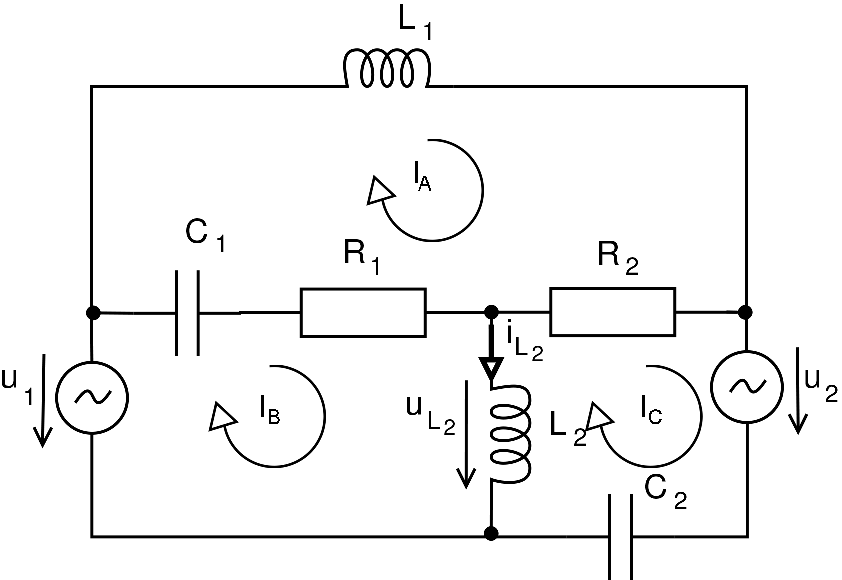
\includegraphics[scale=0.5,keepaspectratio]{sablona/fig/Pr4_Smycky.pdf} 
  \caption{Obvod rozšířený o smyčkové proudy}
\end{figure} %Preeej se bude hodit na další vobrázek s smyčkama <3
\newline

Vypočítáme úhlovou rychlost $\omega$ a impedanci u všech cívek a kondenzátorů:
\newline

$$\omega = 2\pi\mathit{f} = 2\pi*95 = 190\pi = 596,9026042 rad * s^{-1}$$ 
$$Z_{L_1} = j\omega L_1 = j * 596,9026042 * 0,155 = 95,50441667j \Omega$$ 
$$Z_{L_2} = j\omega L_1 = j * 596,9026042 * 0,075 = 44,76769531j \Omega$$
$$Z_{C_1} = -\frac{j}{\omega C_1} = -\frac{j}{596,9026042*0,000155} = -10,80844851j\Omega$$
$$Z_{C_2} = -\frac{j}{\omega C_2} = -\frac{j}{596,9026042*0,000075} = -23,93307415j \Omega$$
\newpage
Dle II. Kirchhofova zákona sestavíme rovnice pro jednotlivé smyčky:
\newline

$$A: I_A(Z_{L_1}+R_1+R_2+Z_{L_2}) + I_B(-Z_{C_1}-R_1) + I_C(-R_2) = 0$$
$$B: I_A(-Z_{L_1}-R_1) + I_B(Z_{C_1}+R_1+Z_{L_2}) + I_C(-Z_{L_2}) = -U_1$$
$$C: I_A(-R_2) + I_B(-Z_{L_2}) + I_C(R_2+Z_{C_2}+Z_{L_2}) = U_2$$
\newline

Dosadíme hodnoty do rovnic:
\newline

$$I_A(20+84,69593157j) + I_B(-10+10,8084851j) + I_C(-10) = 0$$
$$I_A(-10+10,8084851j) + I_B(10+33,95921021j) + I_C(-44,7676953j) = 6$$
$$I_A(-10) + I_B(-44,7676953j) + I_C(10+20,83462115j) = -5$$
\newline

Z rovnic sestavíme matici:

\[
\left(
\begin{array}{ccc}
20+84,69593157j & -10+10,8084851j & -10\\
-10+10,8084851j & 10+33,95921021j & -44,7676953j\\
-10 & -44,7676953j & 10+20,83462115j\\
\end{array}
\right)
*
\left(
\begin{array}{c}
I_A\\
I_B\\
I_C\\
\end{array}
\right)
=
\left(
\begin{array}{c}
0\\
6\\
-5\\
\end{array}
\right)
\]
\newline
\newline

Za pomoci Sarrusova pravidla vypočítáme determinant:
\[
D = 
\left|
\begin{array}{ccc}
20+84,69593157j & -10+10,8084851j & -10\\
-10+10,8084851j & 10+33,95921021j & -44,7676953j\\
-10 & -44,7676953j & 10+20,83462115j\\
\end{array}
\right|
\]
\newline

$$\mathbf{D} = 33488,76035345512 - 119409,4809375206j$$
\newline

Za pomoci Cramerova pravidla vypočítáme $D_{I_B}$ a $D_{I_C}$:
\[
D_{I_B} = 
\left|
\begin{array}{ccc}
20+84,69593157j & 0 & -10\\
-10+10,8084851j & 6 & -44,7676953j\\
-10 & -5 & 10+20,83462115j\\
\end{array}
\right|
\]
\newline

$$\mathbf{D_{I_B}} = 13826,81171073515 + 1594,644363263870j$$

\newpage
\[
D_{I_C} = 
\left|
\begin{array}{ccc}
20+84,69593157j & -10+10,8084851j & 0\\
-10+10,8084851j & 10+33,95921021j & 6\\
-10 & -44,7676953j & -5\\
\end{array}
\right|
\]
\newline

$$\mathbf{D_{I_C}} = -2501,906728286798 - 6517,534055424680j$$
\newline

Vypočítáme proudy $I_B$ a $I_C$, jelikož se jedná o proudy v tento okamžik, tak je budeme označovat jako $i_B$ a $i_C$:
$$i_B = \frac{D_B}{D} = \frac{13826,81171073515 + 1594,644363263870j}{33488,76035345512 - 119409,4809375206j} = -0,923032098009625 + 1,767151716639510j A $$
\newline

$$i_C = \frac{D_C}{D} = \frac{-2501,906728286798 - 6517,534055424680j}{33488,76035345512 - 119409,4809375206j} = 0,743134122177088 + 0,669142493386939j A $$
\newline

Z námi vypočítaných hodnot dopočítáme okamžité napětí $u_{L_2}$:
$$u_{L_2} = Z_{L_2} * (i_B - i_C)$$
$$u_{L_2}= 44,76769531 * (-0,923032098009625 + 1,767151716639510j - (0,743134122177088 + 0,669142493386939j))$$
$$u_{L_2} = 6,466146610661667 + 1,227878191680738jV$$
\newline

Vypočítáme amplitudu na cívce |$u_{L_2}$|:
$$|u_{L_2}| = \sqrt{(6,466146610661667)^2 + (1,227878191680738)^2} = \mathbf{6,581697109726071V}$$
\newline

V poslední řadě vypočítáme fázový posun $\varphi_{L_2}$:
$$\varphi_{L_2} = arctan(\frac{im}{re}) = arctan(\frac{6,466146610661667}{1,227878191680738}) = \mathbf{10,752068858738161Rad}$$
